\documentclass{paper}

%\usepackage{times}
\usepackage{epsfig}
\usepackage{graphicx}
\usepackage{amsmath}
\usepackage{amssymb}
\usepackage{color}
\usepackage{caption}
\usepackage{subcaption}


% load package with ``framed'' and ``numbered'' option.
%\usepackage[framed,numbered,autolinebreaks,useliterate]{mcode}

% something NOT relevant to the usage of the package.
\setlength{\parindent}{0pt}
\setlength{\parskip}{18pt}






\usepackage[latin1]{inputenc} 
\usepackage[T1]{fontenc} 

\usepackage{listings} 
\lstset{% 
   language=Matlab, 
   basicstyle=\small\ttfamily, 
} 



\title{Report Template}



\author{Jenni Simon\\09-116-005}
% //////////////////////////////////////////////////


\begin{document}



\maketitle


% Add figures:
%\begin{figure}[t]
%%\begin{center}
%\quad\quad   \includegraphics[width=1\linewidth]{ass2}
%%\end{center}
%
%\label{fig:performance}
%\end{figure}

\section*{Photometric Stereo (Due on 27/10/2015)}



\paragraph{1. Calibration}

\subparagraph{Algorithm}

Let $r$ be the radius and $c=(c_x,c_y)$ be the image-coordinates of the
sphere. Further let $s_i=(s_{ix},s_{iy})$ be the image-coordinates of the
highlights on the sphere in image $i$ for $i\in{\{1,...N\}}$. Let the
unit vector $d=(0,0,-1)$ denote the direction of the camera from any point on the sphere.
The 3D-coordinates of the surface-normal at a position $p=(p_{x},p_{y})$ on the sphere can then be computed as 
\begin{equation} 
\begin{split}
  n_x(p)  &=  \frac{p_x-c_x}{r}      \\
  n_y (p) &=  \frac{p_y-c_y}{r}      \\
  n_z(p)  &=  -\sqrt{1-n_x^2-n_y^2}   
\end{split}   
\end{equation}

Note that the normal $n(p)=(n_x,n_y,n_z)$ then already has unit length.
The unnormalised directions of the light-sources $L_i$ for $i\in{\{1,...N\}}$ are then given by 
\begin{equation} 
L_i=2\cdot (n(s_i))^Td\cdot n(s_i)-d
\end{equation}


\subparagraph{Resulting Light-Directions} 

Normalising these light-directions I obtained the following results:
\begin{align}
\mathbf{L^T}= \left[ \begin{array}{ccc}
0.496 & -0.466 & -0.733\\
0.245 & -0.129 & -0.961 \\
-0.038 & -0.180 & -0.983 \\
-0.103 & -0.438 & -0.893 \\
-0.323 & -0.506 & -0.799 \\
-0.117 & -0.558 & -0.822 \\
0.287 & -0.418 & -0.862 \\
0.094 & -0.438 & -0.894 \\
0.209 & -0.342 & -0.916 \\
0.095 & -0.327 & -0.940 \\
0.129 & -0.046 & -0.990 \\
-0.136 & -0.359 & -0.923 
\end{array} \right] \nonumber
\end{align}



\paragraph{2. Computing Surface Normals and Grey Albedo}


\begin{figure*}[h!]
    \centering
    \begin{subfigure}[]{0.33\textwidth}
        \centering
        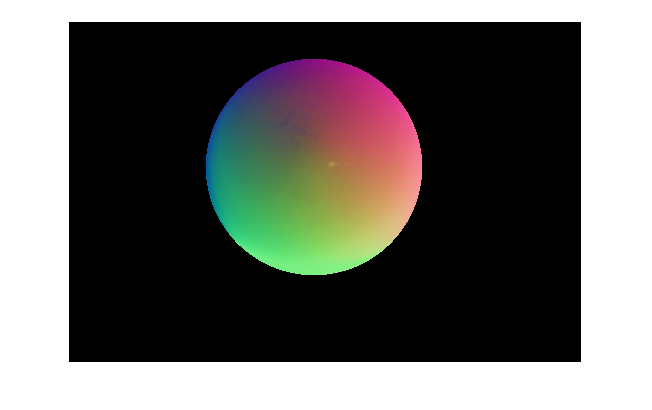
\includegraphics[height=1.2in]{sphereNM}
    \end{subfigure}%
    ~ 
    \begin{subfigure}[]{0.33\textwidth}
        \centering
        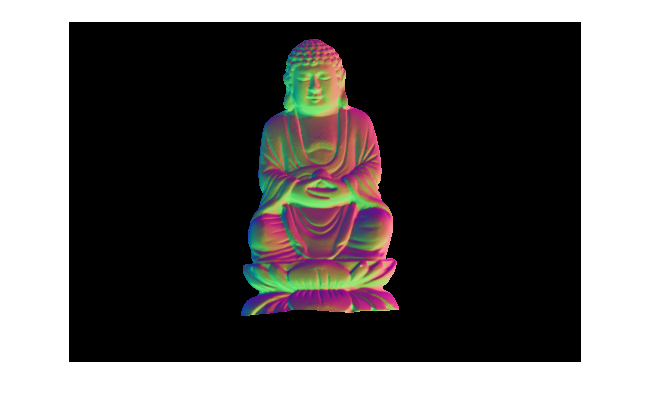
\includegraphics[height=1.2in]{buddhaNM}
    \end{subfigure}%
    ~ 
    \begin{subfigure}[]{0.33\textwidth}
        \centering
        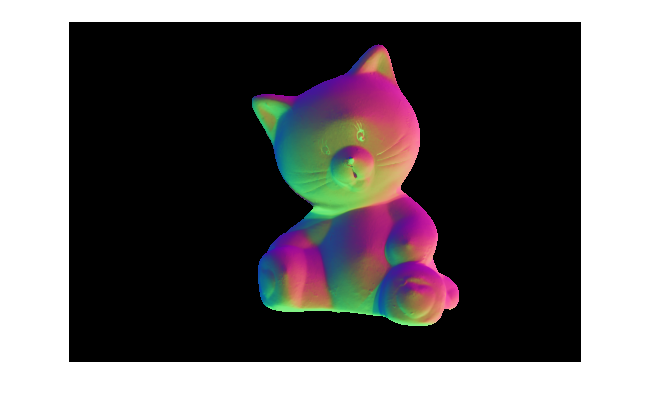
\includegraphics[height=1.2in]{catNM}
    \end{subfigure}
        \begin{subfigure}[]{0.33\textwidth}
        \centering
        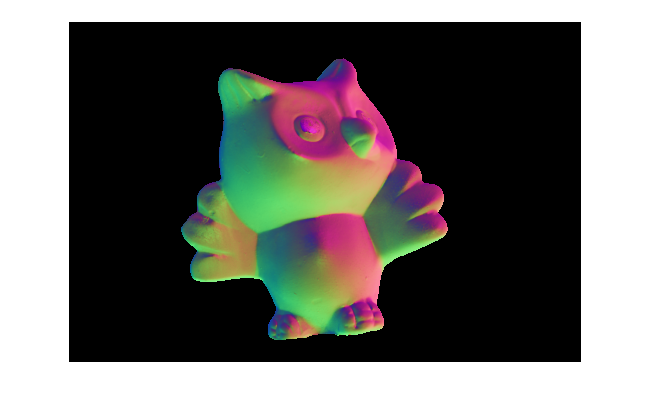
\includegraphics[height=1.2in]{owlNM}
    \end{subfigure}%
    ~ 
    \begin{subfigure}[]{0.33\textwidth}
        \centering
        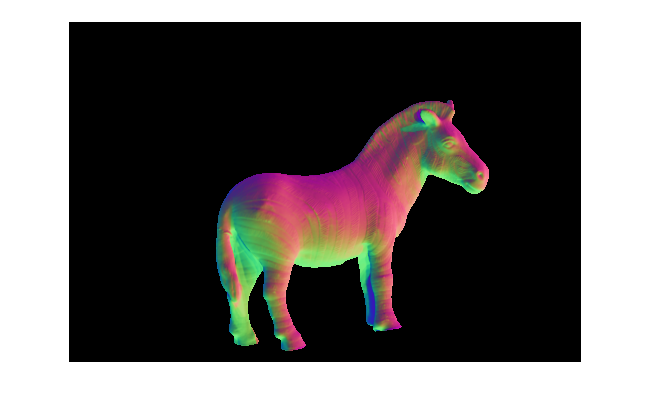
\includegraphics[height=1.2in]{zebraNM}
    \end{subfigure}%
    ~ 
    \begin{subfigure}[]{0.33\textwidth}
        \centering
        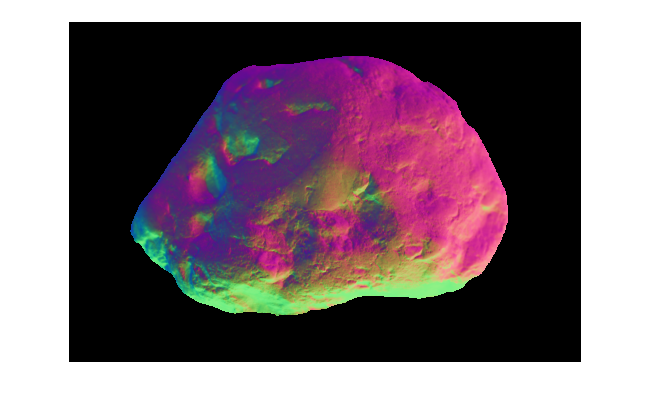
\includegraphics[height=1.2in]{rockNM}
    \end{subfigure}

    \caption{Normal maps}    
\end{figure*}

\begin{figure*}[h!]
    \centering
    \begin{subfigure}[]{0.33\textwidth}
        \centering
        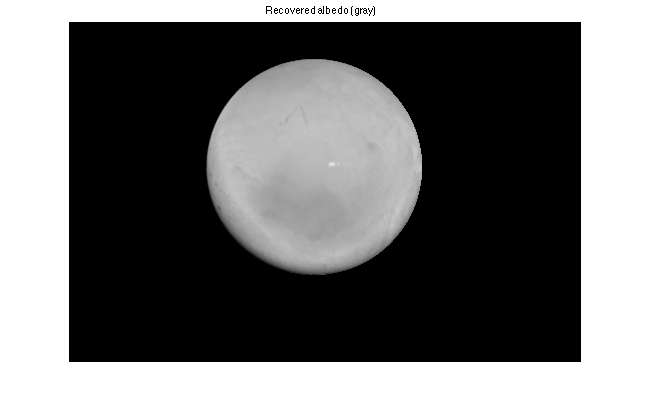
\includegraphics[height=1.2in]{sphereGA}
    \end{subfigure}%
    ~ 
    \begin{subfigure}[]{0.33\textwidth}
        \centering
        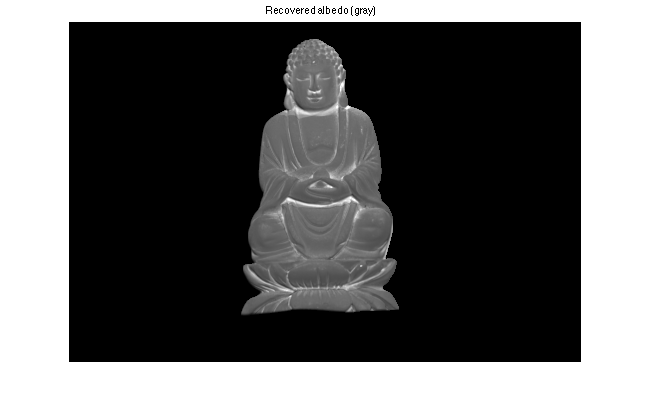
\includegraphics[height=1.2in]{buddhaGA}
    \end{subfigure}%
    ~ 
    \begin{subfigure}[]{0.33\textwidth}
        \centering
        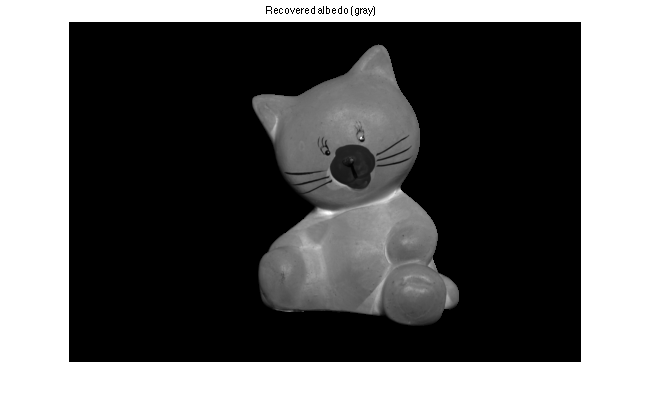
\includegraphics[height=1.2in]{catGA}
    \end{subfigure}
        \begin{subfigure}[]{0.33\textwidth}
        \centering
        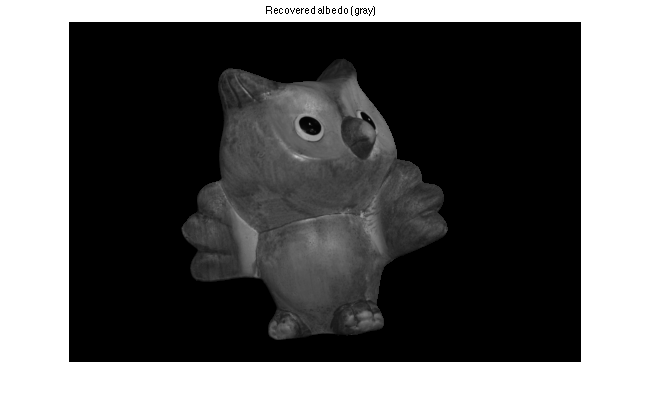
\includegraphics[height=1.2in]{owlGA}
    \end{subfigure}%
    ~ 
    \begin{subfigure}[]{0.33\textwidth}
        \centering
        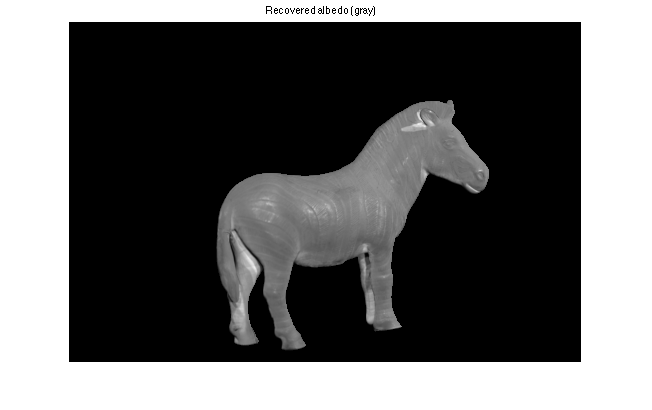
\includegraphics[height=1.2in]{zebraGA}
    \end{subfigure}%
    ~ 
    \begin{subfigure}[]{0.33\textwidth}
        \centering
        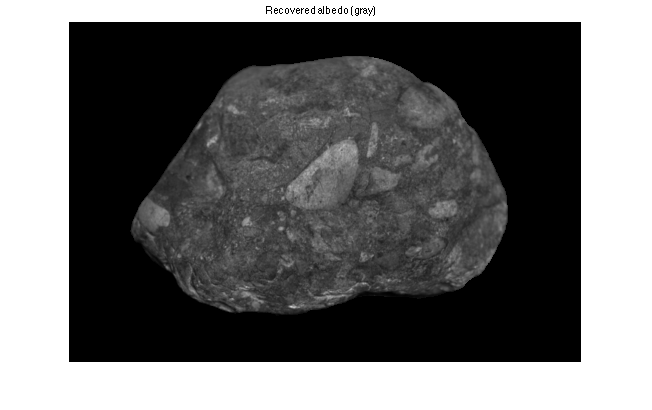
\includegraphics[height=1.2in]{rockGA}
    \end{subfigure}

    \caption{Recovered gray albedo}    
\end{figure*}


\begin{figure*}[h!]
    \centering
    \begin{subfigure}[]{0.33\textwidth}
        \centering
        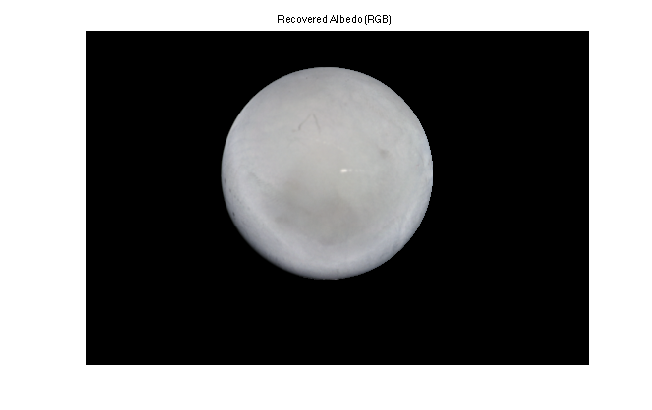
\includegraphics[height=1.2in]{sphereRGB}
    \end{subfigure}%
    ~ 
    \begin{subfigure}[]{0.33\textwidth}
        \centering
        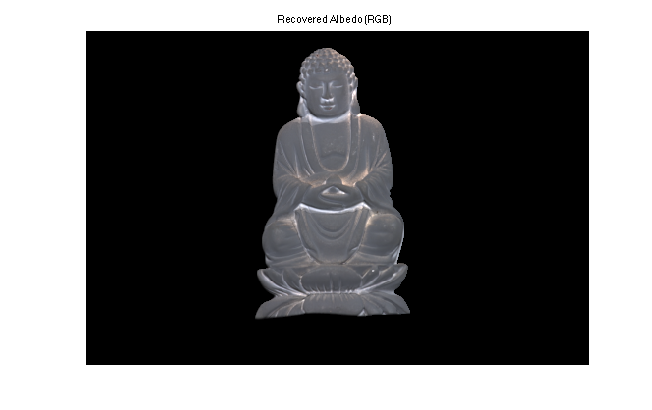
\includegraphics[height=1.2in]{buddhaRGB}
    \end{subfigure}%
    ~ 
    \begin{subfigure}[]{0.33\textwidth}
        \centering
        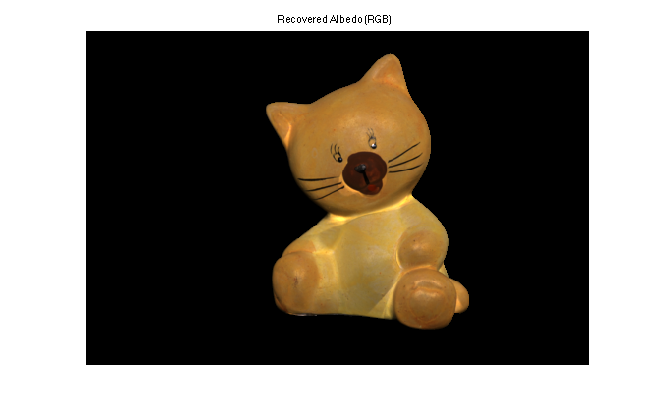
\includegraphics[height=1.2in]{catRGB}
    \end{subfigure}
        \begin{subfigure}[]{0.33\textwidth}
        \centering
        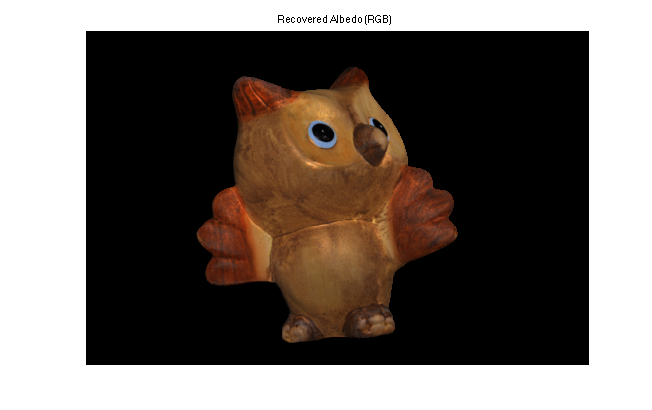
\includegraphics[height=1.2in]{owlRGB}
    \end{subfigure}%
    ~ 
    \begin{subfigure}[]{0.33\textwidth}
        \centering
        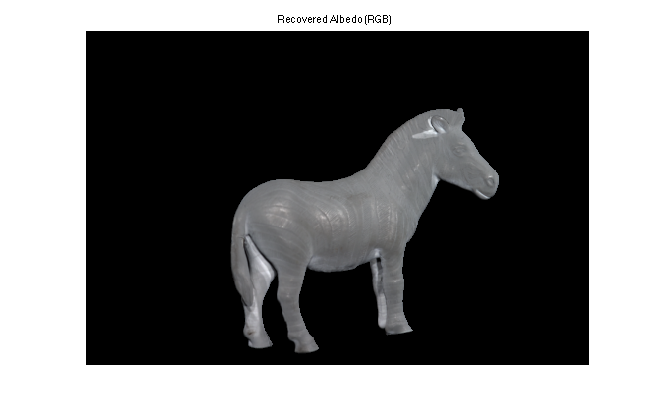
\includegraphics[height=1.2in]{zebraRGB}
    \end{subfigure}%
    ~ 
    \begin{subfigure}[]{0.33\textwidth}
        \centering
        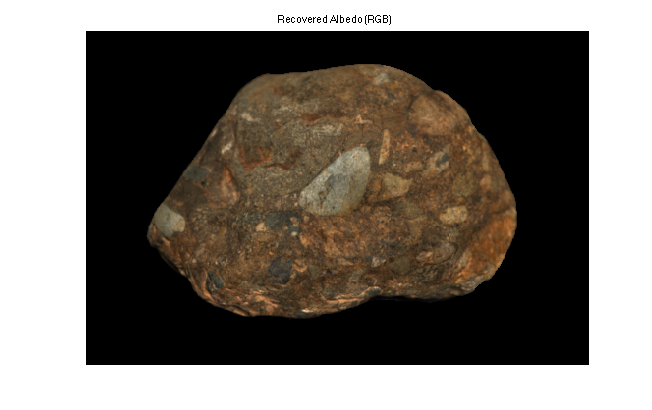
\includegraphics[height=1.2in]{rockRGB}
    \end{subfigure}

    \caption{Recovered RGB albedo}    
\end{figure*}


\begin{figure*}[h!]
    \centering
    \begin{subfigure}[]{0.33\textwidth}
        \centering
        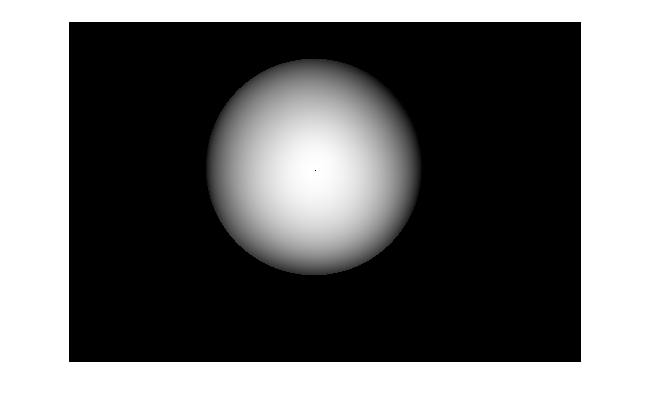
\includegraphics[height=1.2in]{sphereDM}
    \end{subfigure}%
    ~ 
    \begin{subfigure}[]{0.33\textwidth}
        \centering
        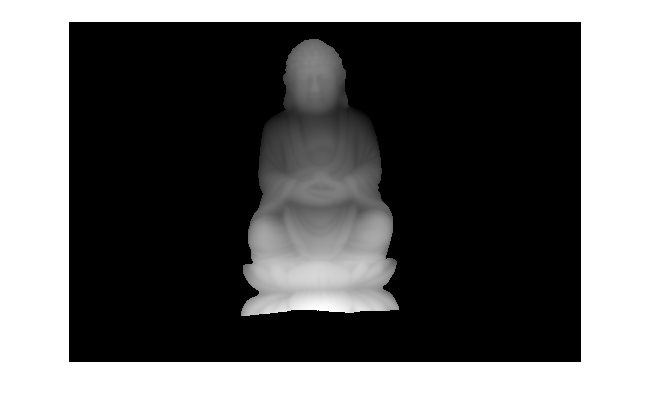
\includegraphics[height=1.2in]{buddhaDM}
    \end{subfigure}%
    ~ 
    \begin{subfigure}[]{0.33\textwidth}
        \centering
        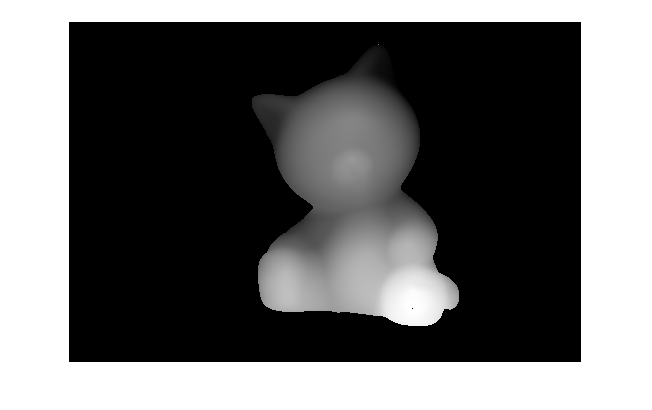
\includegraphics[height=1.2in]{catDM}
    \end{subfigure}
        \begin{subfigure}[]{0.33\textwidth}
        \centering
        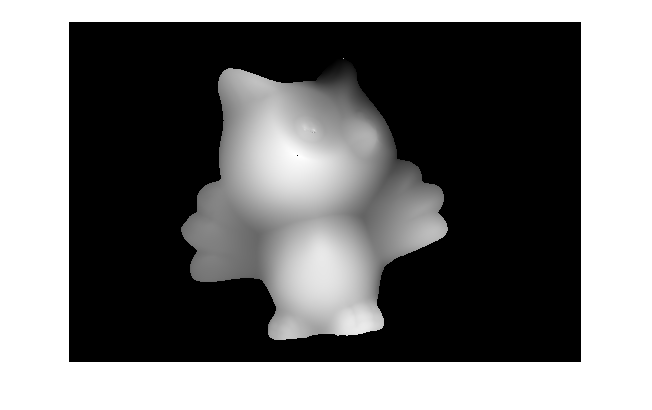
\includegraphics[height=1.2in]{owlDM}
    \end{subfigure}%
    ~ 
    \begin{subfigure}[]{0.33\textwidth}
        \centering
        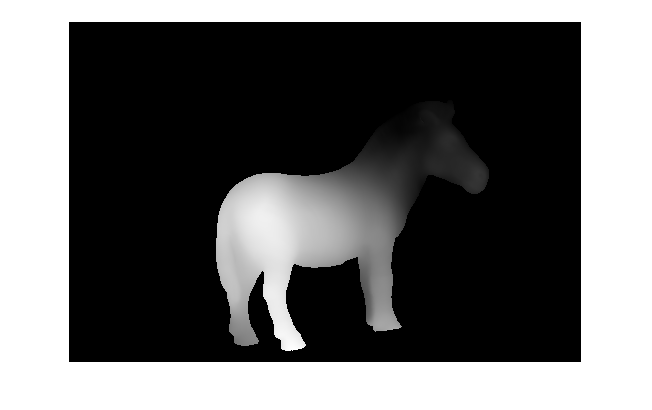
\includegraphics[height=1.2in]{zebraDM}
    \end{subfigure}%
    ~ 
    \begin{subfigure}[]{0.33\textwidth}
        \centering
        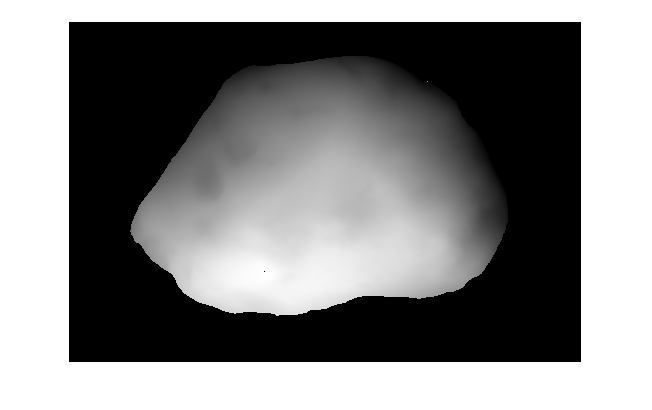
\includegraphics[height=1.2in]{rockDM}
    \end{subfigure}

    \caption{Recovered RGB albedo}    
\end{figure*}




In this section you should:

\begin{itemize}
\item Describe the algorithm you used for calculating the albedo and normals given the light directions you estimated (or the approximated one which is provided in case you did not complete the task 1). You need to provide the formula you used to calculate the normals.

\item Display the image of the recovered grayscale albedo map for each dataset.
\item Display the images of the three normal components (x,y and z directions) or a single colour image with the x,y and z components instead of the R,G, and B components rispectively.
\item Display the image of the RGB albedo map for each dataset. 
\end{itemize}



\paragraph{3. Surface Fitting (35 points)}

In this section you should:

\begin{itemize}
\item Describe the algorithm you used for calculating the depth map given the normals you calculated before.
\item Display the image of the depth map (in colour or grayscale) for each dataset, where higher intensity values indicate points closer to the camera.
\item Describe, in no more than a few paragraphs, your assessment of when the technique works well, and when there are failures. When the technique fails to produce nice results, please explain as best as you can what the likely causes of the problems are.
\end{itemize}















 \end{document}